\chapter{Dati utilizzati}
\label{chap:dati}

Il progetto ICOS fornisce dati standardizzati e di altas qualità sui gas a effetto serra.
Tutti i dati sono accessibili attraverso la licenza \textit{Creative Commons Attribution 4.0 International license}.
La licenza Creative Commons 4.0 permette di condividere e utilizzare opere originali in modo più flessibile rispetto
al diritto d'autore tradizionale, ma con alcune limitazioni e requisiti per garantire il rispetto dei diritti dell'autore originale.

\section{FAIR principles}
\label{section:fair}
I dati prodotti da ICOS seguono i cosidetti principi \textbf{FAIR}.
I principi FAIR mirano a fornire all'utente strumenti sufficienti per 
comprendere il significato dei dati prima e dopo averli scaricati. 
I principi FAIR definiscono quindi dei requisiti fondamentali per
la gestione dei dati scientifici, al fine di renderli "FAIR",
ovvero Findable (Rintracciabili), Accessible (Accessibili), Interoperable (Interoperabili) e 
Reusable (Riutilizzabili). A tale scopo, ICOS utilizza la tecnologia dei \textit{Linked-Open Data} \ref{section:linkeddata},
tecnologia moderna e avanzata nel campo della gestione dati. 

I quattro principi FAIR sono i seguenti:

\begin{itemize}
    \item Findable: i dati scientifici devono essere facilmente identificabili e rintracciabili attraverso i metadati appropriati.
    Ciò implica l'utilizzo di identificatori univoci e di descrizioni dettagliate dei dati.
    \item Accessible: i dati scientifici devono essere accessibili in modo aperto e gratuito.
    Ciò implica l'utilizzo di licenze adeguate e la disponibilità di strumenti e tecnologie per accedere ai dati.
    \item Interoperable: i dati scientifici devono essere interoperabili, ovvero strutturati in modo standard
    e condivisibili con altre fonti di dati. Ciò implica l'utilizzo di formati standard, di ontologie e di protocolli
    di comunicazione comuni.
    \item Reusable: i dati scientifici devono essere riutilizzabili
    in modo flessibile e senza restrizioni, anche per scopi diversi da quelli
    per cui sono stati creati. Ciò implica la pubblicazione di dati e metadati completi,
    la documentazione dei processi di acquisizione e la creazione di strutture di dati flessibili.
\end{itemize}


\section{PIDs}
Per collegare la proprietà dei dati al dato stesso, ICOS impiega i \textbf{Persistent Identifiers (PIDs)}.
Questo identificatore univoco utilizza i \textit{DataCite Digital Object Identifiers (DOIs)} per i datasets
e le collezioni. Questi tag identificano ciascuno \textit{data object} e può essere citato, per esempio,
in una qualche pubblicazione scientifica. Il PID è creato automaticamente e immediatamente
non appena il data è caricato; inoltre il dato viene cifrato per assicurarne la validità.\\

Il PID è un indirizzo web valido (URL), che riporta ad una sua specifica landing page,
dove molteplici informazioni possono essere trovate tra cui i meta-data accessibili sia
dagli utenti che dalle macchine. L'intero processo garantisce che il dato scaricato e quello
originale sia esattamente identici con i metadati associati. Altri portali 
potrebbero usare il PID e il link associato al dato e fornire accesso trasparente al \textit{data object}
attraverso l'ICOS Carbon Portal.

\begin{figure}[h!]
    \centering
    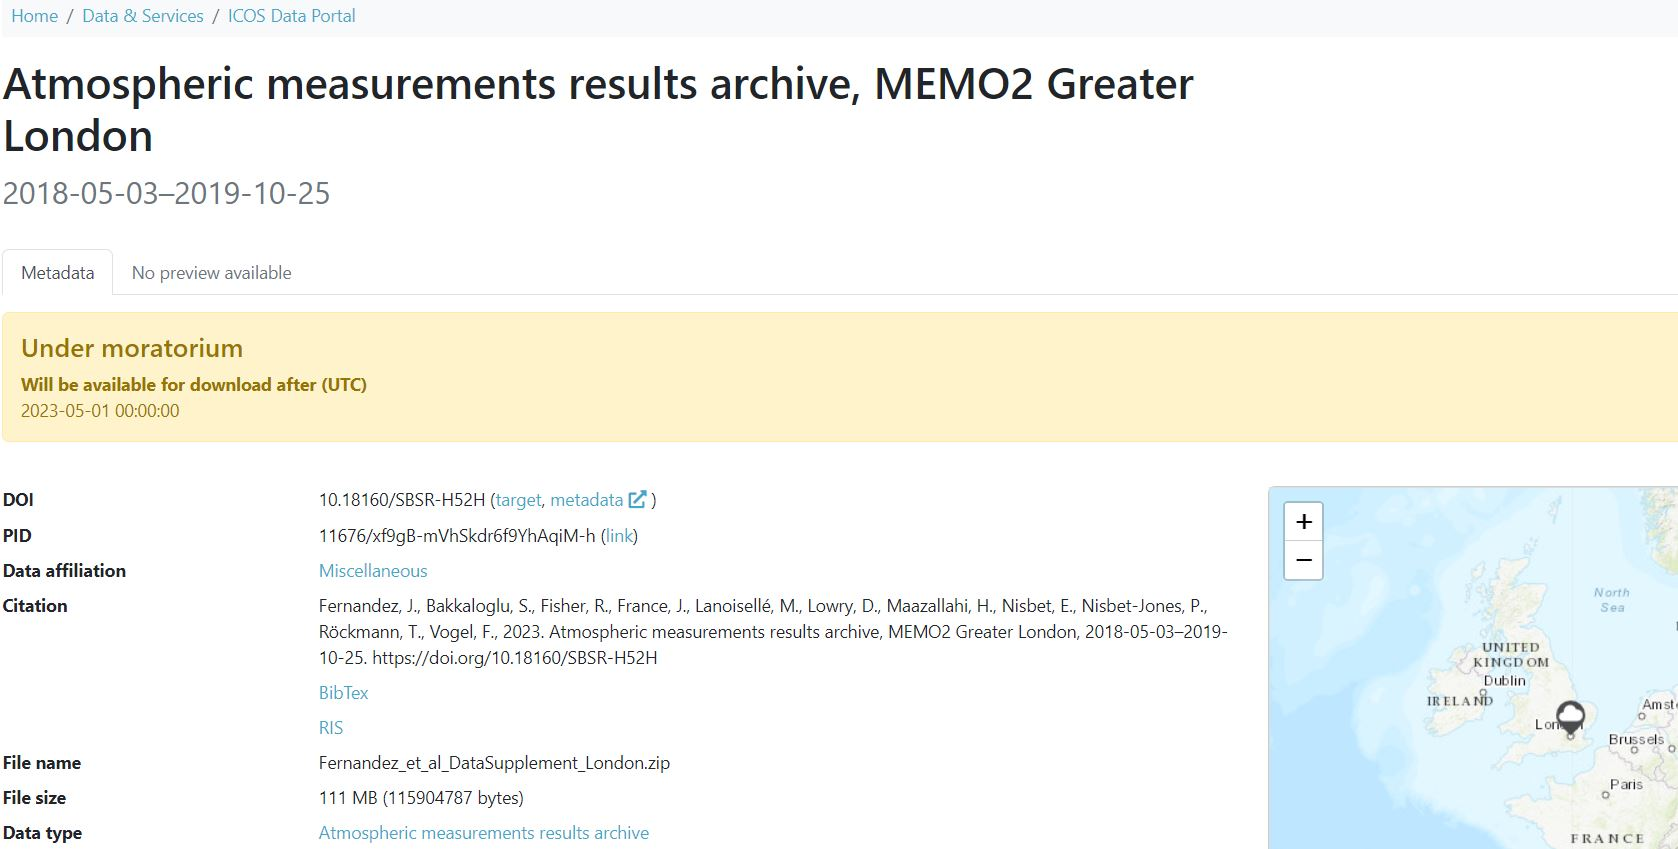
\includegraphics[width=0.7\textwidth]{figures/PIDex.JPG}
    \caption{Esempio di pagina web contentente i metadati tra cui il PID (il link della pagina) e il DOI.}
    \label{figure:PIDex}
\end{figure}

\begin{figure}[h!]
    \centering
    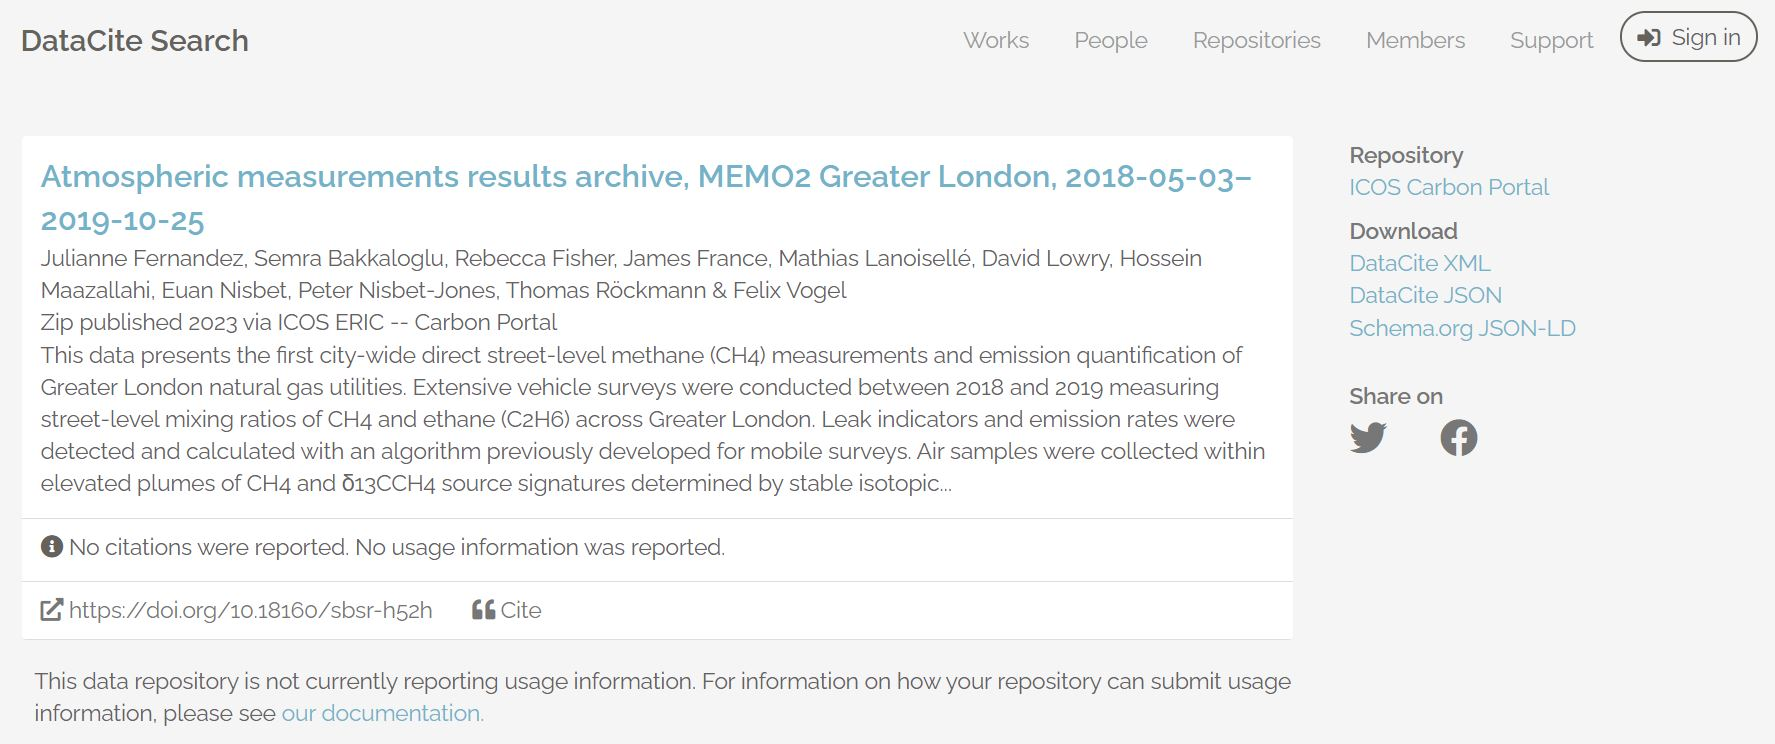
\includegraphics[width=0.7\textwidth]{figures/DOIex.JPG}
    \caption{Esempio di DOI che riporta automaticamente ad una risorsa all'intereno del dominio di DataCite.}
    \label{figure:DOIex}
\end{figure}


\section{Data-production Process}
Il processo di produzione e standardizzazione dei dati segue 11 fasi, descritte qui di seguito e nella figura \ref{figure:data-process}:
\begin{enumerate}
    \item \textit{I dati son raccolti presso le stazioni di misurazione}.
    ICOS possiede circa 150 stazioni di misurazione, suddivisi in 14 paesi,
    che formano tre reti principali di raccolta (\ref{section:thematic}, Atmosphere, Ecosystem e Ocean).
    \item \textit{I dati grezzi vengono salvati in repository sicure}.
    Essendo i dati il fulcro di questo progetto, inoltre è impossibile raccogliere nuovamente
    lo stesso dato, i dati vengono salvati entro 24 ore all'interno di
    data center sicuri.
    \item \textit{I dati vengono inoltrati al centro di interesse}. Ogni stazione manda i dati dei propri sensori al centro di interesse
    (\ref{section:thematic}, Atmosphere, Ecosystem o Ocean), che li processano ulteriormente e su cui svolgono controlli di qualità.
    \item \textit{I dati sono inoltre inviati al CAL}. Il CAL (\ref{section:CAL}, Central Analytical Laboratories)
     ha come obiettivo quello di garantire
    l'accuratezza delle misure atmosferiche nelle stazioni ICOS.
    \item \textit{Il centro di interesse elabora i dati}. Il centro di interesse che riceve i dati dovrà controllare la validità dei dati, assicurarne la qualità e
    standardizzarli. Infine, i dati vengono aggregati in gruppi di misurazioni da mezz'ora o un'ora.
    \item \textit{Dato trasferiti al Carbon Portal}. Quando i dati sono pronti vengono inviati al Carbon Portal \ref{section:carbonportal}, 
    cercando giorno dopo giorno d ridurre i tempi di delivery di questi dati.
    \item \textit{Il Carbon Portal riceve e si prende cura di tutti i datasets ICOS}. Il Carbon Portal \ref{section:carbonportal} si occuperà della gestione, dei servizi di visualizzazione e data management legati ai datasets ICOS.
    \item \textit{Gli utenti possono liberamente agire sui dati}. Chiunque voglia accedere, scaricare e visualizzare i dati potrà farlo dal Carbon Portal \ref{section:carbonportal}.
    \item \textit{Tutti gli ICOS Data Products sono in data center sicuri}. Copie di tutti i Data Product, e i relativi metadati,
    sono salvati in maniera sicura in repository dislocate geograficamente (Finalndia, Germania e centro tematico d'iteresse).
    \item \textit{Le descrizioni dei Data Products devono essere facilmente accessibili}. ICOS si impegna a diffondere tutte le informazioni relative ai Data Product.
    \item \textit{I dati ICOS devono essere inviabili agli altri centri di ricerca}. Il processo e le infrastrutture per la produzione dei dati ICOS devono fare in modo che i dati prodotti possano essere facilmente 
    trasferibili ad altri centri di ricerca che potrebbero beneficiarne.
\end{enumerate}

\begin{figure}[h!]
    \centering
    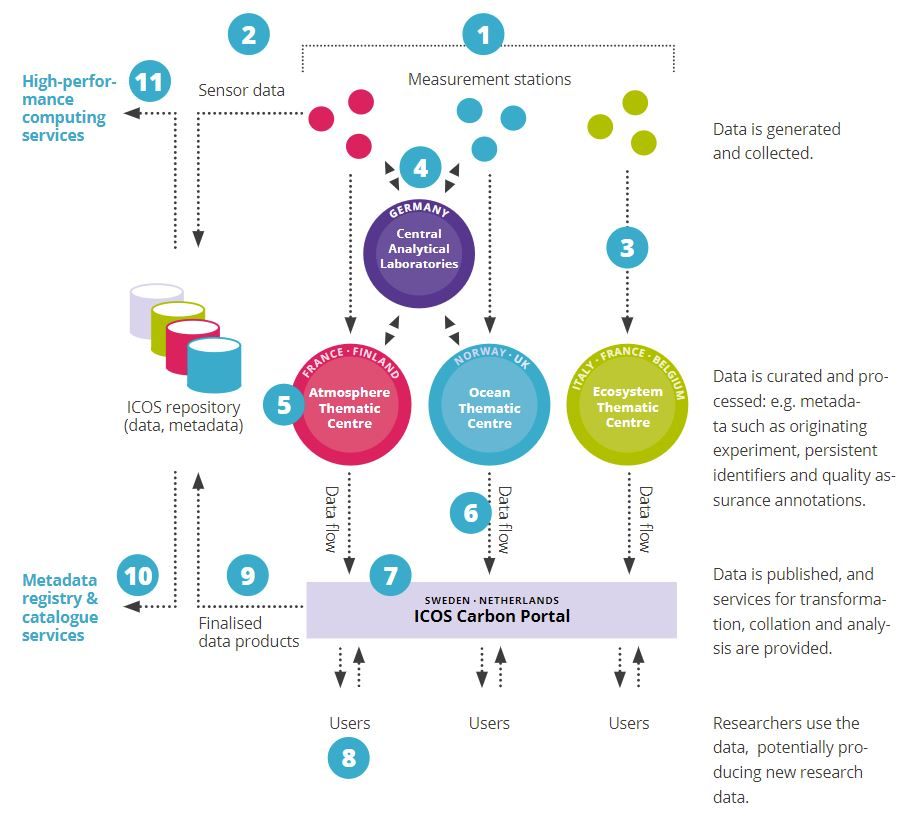
\includegraphics[width=0.8\textwidth]{figures/data-process.JPG}
    \caption{Diagramma della processo di produzione e mantenimento dei dati ICOS.}
    \label{figure:data-process}
\end{figure}


\section{Data product levels}
\label{section:data-level}
Per definire al meglio quelli che ICOS considera dati "grezzi" da dati "finiti",
questi dati sono stati raggruppati in 4 possibili livelli, a seconda della qualità.

\begin{enumerate}
    \item \textbf{Dati grezzi}. Sono i dati direttamente raccolti dai sensori delle stazioni e quindi non elaborati. Possono assumere diverse forme come immagini, testo o campioni fisici.
    \item \textbf{Livello Dati 0}. I dati di livello 0
    sono dati in unità fisiche forniti direttamente dagli
    strumenti o convertiti manualmente dal reparto
    ingegneristico (ad esempio, mV, mA) in unità fisiche
    del Centro Tematico. Potrebbero esserlo stati
    filtrati da un primo controllo qualitativo.
    \item \textbf{Livello Dati 1}. I dati di livello 1 si dividono in due sotto categorie:
        \begin{itemize}
            \item \textit{Level 1 Near Real Time data (L1\_NRT)}. Sono dati che 
            vengono generalmente distribuiti entro 24 ore dalla rilevazione,
            raggruppati in dataset di alta qualità (che quindi hanno superato
            controlli di qualità) e resi disponibili automaticamente attraverso
            il Carbon Portal.  
            \item \textit{Level 1 Internal or Intermediate Working data (L1\_IW)}.
            Questi dati sono generati dagli step intermedi per la preparazione dei dati
            NRT o di livello 2. Per questo motivo non verranno distribuiti ma rimarranno
            all'interno delle infrastrutture ICOS per controlli di qualità interni
            e torneranno utili nella produzione dei dati di livello 2.
        \end{itemize} 
    \item \textbf{Livello Dati 2}. Sono i dati finali rilasciati da ICOS dopo i più rigorosi
    controlli, accessibili sul Carbon Portal.
    \item \textbf{Livello Dati 3}. Tutti i risultati prodotti da ricercatori o enti
    terzi, quindi esterni ad ICOS, tramite dati ICOS vengono catalogati come dati di livello 3.
\end{enumerate}

\begin{figure}[h!]
    \centering
    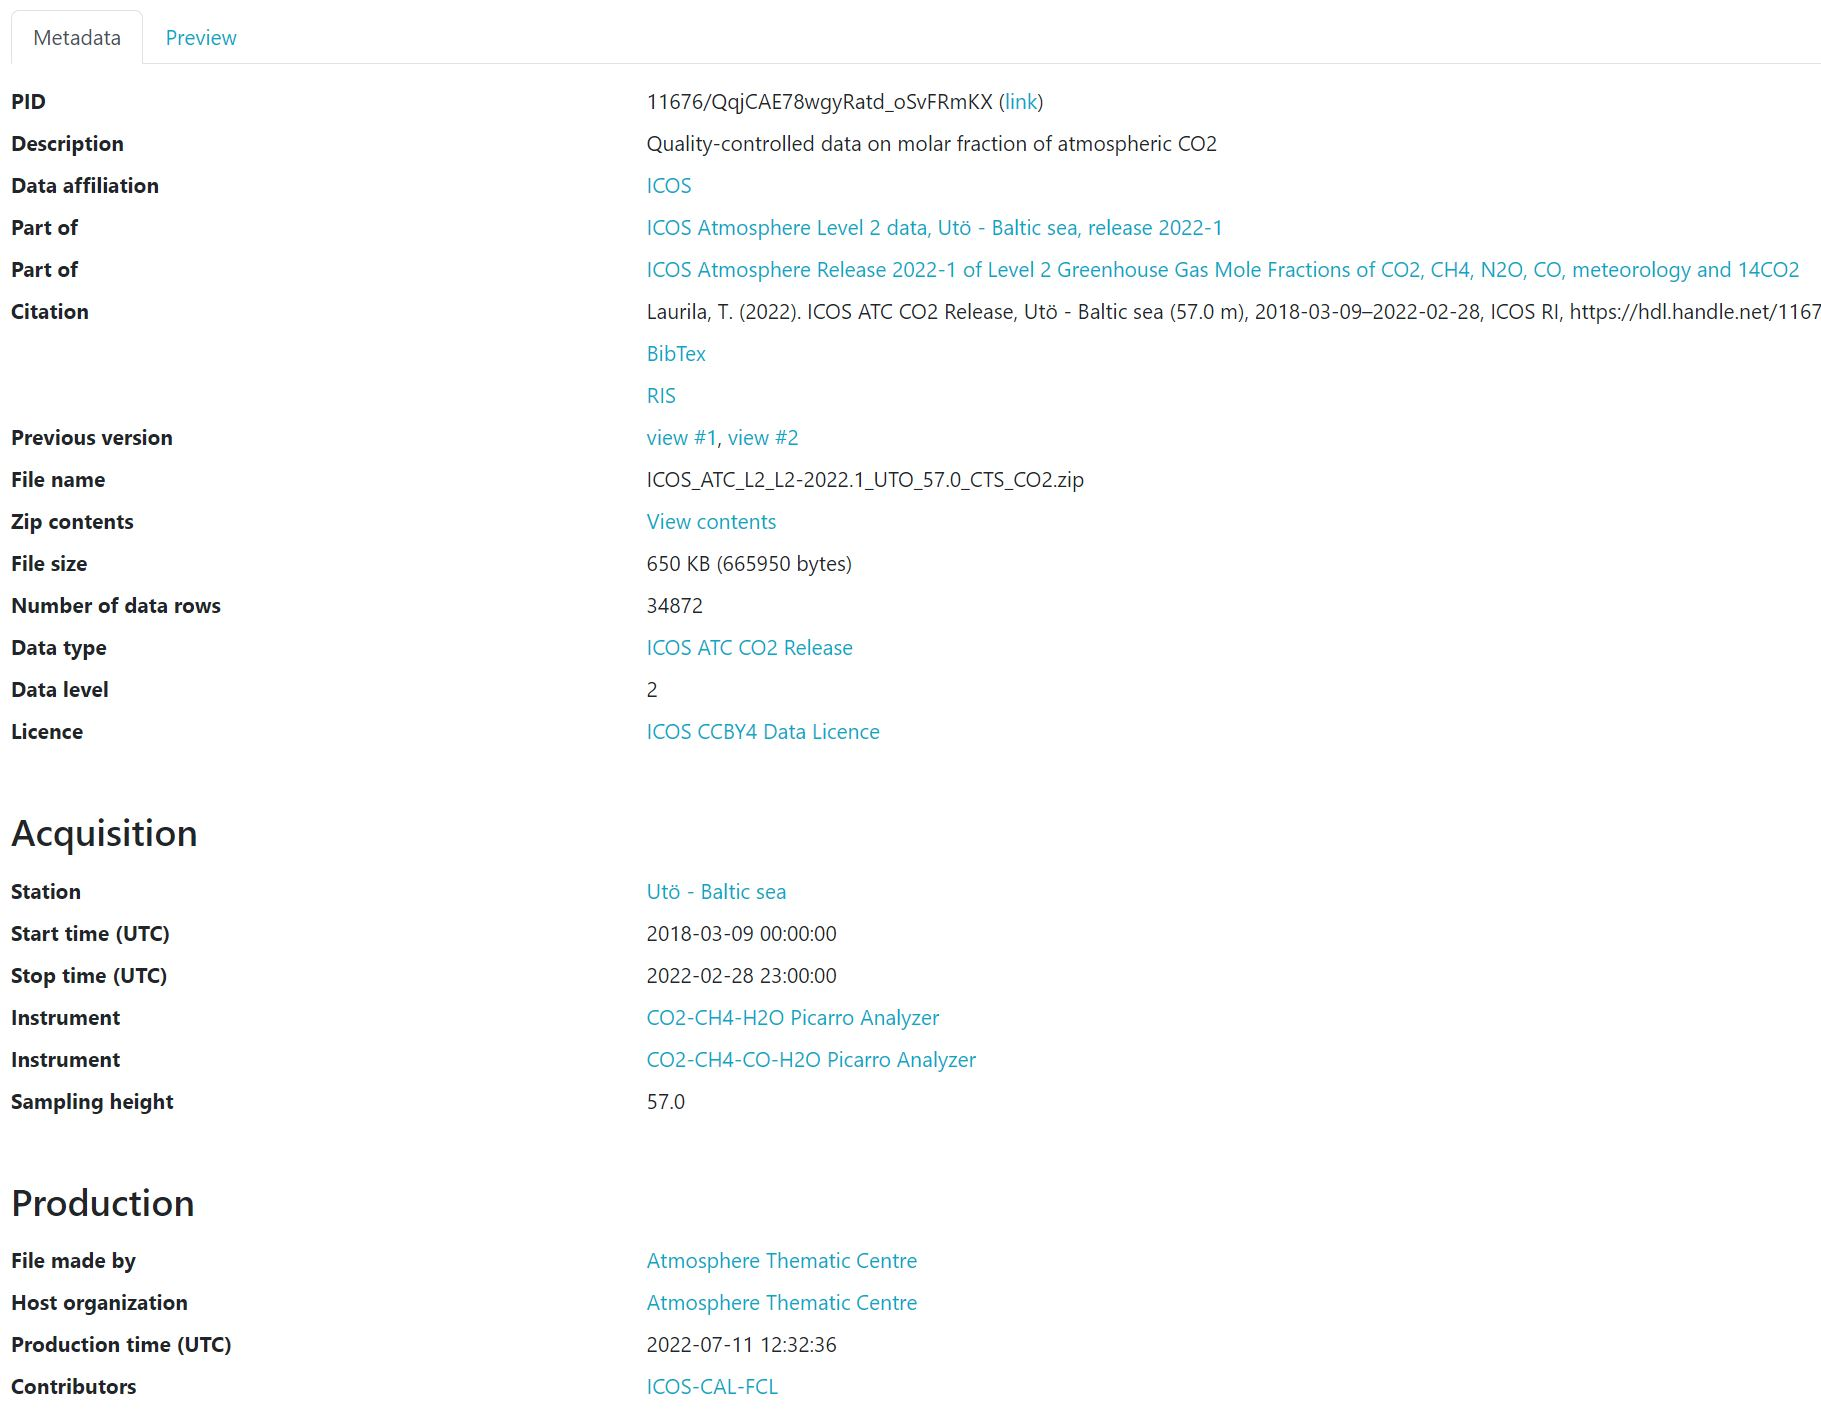
\includegraphics[height=0.36\textwidth]{figures/metaEx.JPG}
    \caption{Alcuni dei meta-data che si possono trovare nei dati ICOS: in figura si può notare tra le altre, anche il Data Level.}
    \label{figure:metadata-ex}
\end{figure}